\documentclass[journal]{IEEEtran}
\usepackage[utf8]{inputenc}
\usepackage[spanish]{babel}
\usepackage{amsmath}
\usepackage{amsfonts}
\usepackage{amssymb}
\usepackage{graphicx}
\usepackage{float}
\author{Cesar Mauricio Forero Cardozo}
\title{Algoritmo PSO aplicado a Busqueda y Rescate con Drones en Zonas de Gran Superficie }
\begin{document}
\maketitle
\begin{abstract}
El presente articulo busca brindar una solución eficiente y efectiva para el apoyo en labores de busqueda y rescate en lugares de dificil recorrido. Esto haciendo uso de un ``Enjambre de Drones'' controlados mediante algoritmos comportamentales de PSO que resulten en una alternatia mucho más economica que los protocolos de rescate actualmente usados.\\

Así pues el principal objetivo es optimizar los gastos economicos que las instituciones deberían de emplear para llevar a cabo rescates de personas perdidas en cualquier tipo de terreno, ademas de disminuir tambien el tiempo de busqueda mediante esfuerzos combinados de hombre-maquina aumentando así las probabilidades de supervivencia de las personas perdidas.
\end{abstract}
\section{Introducción}
Según el ministerio de ambiente de Colombia, la cantidad creciente de personas (residentes y extranjeras) que acuden a los parques nacionales del país desde el 2015 ha causado, como es de suponer, un aumento proporcional en la cantidad de personas que se extravían en los territorios de los mismos; por esta razón el Minambiente ha obligado a los turistas a adquirir polizas de seguro que cubran los gastos de los protocolos establecidos para busqueda y rescate.\\

Los costos de los rescates varian de acuerdo a la complejidad geografica, la cantidad de personas perdidas, las condiciones climatologicas y varios factores más que hacen imposibe estimar un presupuesto previo al rescate. Estos factores tambien afectan directamente el tiempo que se deba emplear en la busqueda de los individuos.\\

Actualmente se emplean metodologias de busqueda especializadas que mezclan componentes empiricos y teoricos con el fin de optimizar el rendimiento de los protocolos de busqueda y rescate, sin embargo se esta comenzando a implementar nuevas tecnologias que aceleren el proceso, como por ejemplo uso de naves no tripuladas, simulaciones computacionales e incluso seguimiento satelital.\\

\section{Metodos tipicos de Busqueda y Rescate}
\subsection{Caracterización}
El primer paso para llevar a cabo un rescate efectivo es la caracterización de el personal que se extravio, así como la zona en la que sucedio, esto con el fin de abstraer cierta información crucial para comenzar la busqueda y que resultarán en delimitaciones y priorizaciones de las areas de busqueda.\\

Uno de los criterios más importantes a tener en cuenta es la edad de la persona extraviada, esto debido a que este rasgo en particular nos puede dar una referencia comportamental y psicologicas en general pudiendo deducir las probabilidades de encontrarles en ciertos tipos de lugares.\\

Para los niños entre 4 y 6 años (ver Fig. 1) que se encuentran en su etapa preoperatoria, ya entienden las relaciones de causa y efecto, por lo que su tendencia es la de ir por sennderos y cominos, sin embargo de llegar a alterarse pueden desorientarse y alejarse de dichos puntos .\\

\begin{figure}[H]
\begin{center}
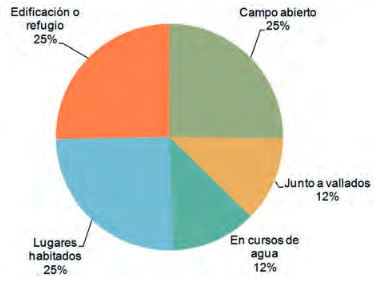
\includegraphics[width=0.35\textwidth]{4a6}
\label{fig:Figure 01}
\textbf{\caption{``Probabilidad de localización niños entre 4 a 6 Años''}}
\end{center}
\end{figure}

Para los niños entre 7 a 12 años (ver Fig. 2) dada su mayor capacidad de orientación, les resulta más facil conservar la calma, orientarse y volver de regreso al punto de partida (ULC).\\

\begin{figure}[H]
\begin{center}
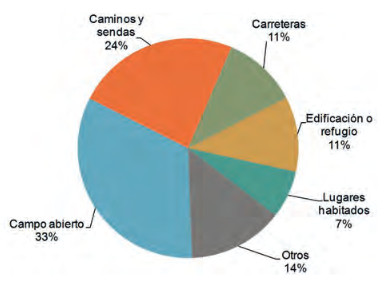
\includegraphics[width=0.35\textwidth]{7a12}
\label{fig:Figure 02}
\textbf{\caption{``Probabilidad de localización niños entre 7 a 12 Años''}}
\end{center}
\end{figure}

En la edad entre 13 a 17 años (ver Fig. 3) el niño tendera a moverse a zonas en donde pueda adquirir mayor información para tomar decisiones a cerca de donde moverse, p.e. lugares altos o poblados.\\

\begin{figure}[H]
\begin{center}
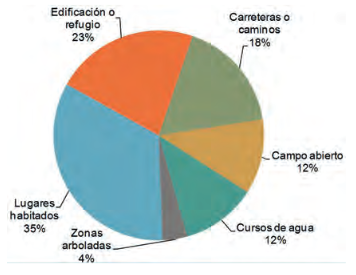
\includegraphics[width=0.35\textwidth]{13a17}
\label{fig:Figure 03}
\textbf{\caption{``Probabilidad de localización niños entre 13 a 17 Años''}}
\end{center}
\end{figure}

Para un adulto (ver Fig. 4), debido a que la causa más probable de perdida sea la de tomar un camino por error, la confianza en su propia cognición y su incapacidad de admitir equivocaciones hacen que el individuo tienda a alejarse mas del ULC.\\

\begin{figure}[H]
\begin{center}
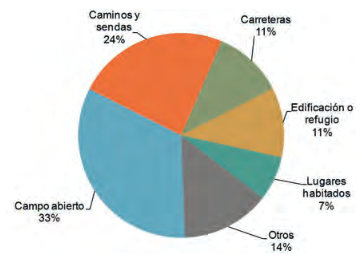
\includegraphics[width=0.35\textwidth]{18oMas}
\label{fig:Figure 04}
\textbf{\caption{``Probabilidad de localización adultos mayores a 18 Años''}}
\end{center}
\end{figure}

\subsection{ULC y radio de busqueda}
Según los protocolos actuales de busqueda y rescate, el primer acercamiento que se debe realizar tras la carecterización es el establecimiento de el "Ultimo Lugar Conicido" (ULC) de la persona perdida; a partir de este y con criterios preestablecidos según la condición física y psicologica del individuo, se determina un radio a traves del que la persona pudo haberse desplazado en linea recta (ver Fig. 5), en este punto estos acercamientos se realizan independientemente de la geologia del terreno.


\begin{figure}[H]
\begin{center}
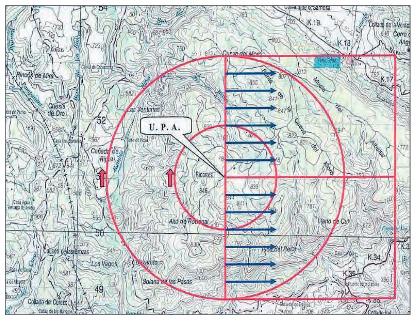
\includegraphics[width=0.35\textwidth]{Radio_SnR}
\label{fig:Figure 5}
\textbf{\caption{``Radio de busqueda determinadas desde el ULC''}}
\end{center}
\end{figure}

Vale la pena resaltar que este método es completamente empírico dependiente en gran manera de la experticia que posea la cabeza del equipo de busqueda y rescate; además las áreas que se obtienen aumentan de manera exponencial conforme pasa el tiempo, dificultando la busqueda de una manera gradual.

\subsection{Busquedas con Drones en la Actualidad}
Actualmente la busqueda de grandes áreas con drones se lleva a cabo de manera mecanica y predefinida; los drones patrullan en la manera que se dispongan en el programa, de manera paralela con camaras de calor o de alta definición y enviando las señales captadas a la central para un análisis manual.\\

Este mécanismo (la busqueda con naves no tripuladas) más que usarse como medio principal, se usa como una metodología de apoyo para ir descartando zonas de patrullaje de manera paulatina pero sin una supervisión automatizada.\\

Al contrario de los excesivos costos de un rescate con vehiculos aereos tripulados, que se encuentran sobre los 4000 euros o 15 millones de pesos colombianos (tan solo el despliegue), la comodidad de transporte y despegue de los drones ademas de funcionar con batería los hacen extremadamente economicos para este proposito, y por ende una opción tentativa muy viable. 

\section{PSO en busqueda y rescate}

\subsection{Algoritmo PSO}

Optimización por Enjambre de Particulas o PSO por sus siglas en ingles (\textit{Particle Swamp Optimization}), es un algoritmo que se basa en el movimiento de las particulas sobre un espacio y su comunicación para encontrar óptimos locales y compararlo con los encontrados por otros componentes del enjambre para así llegar a una notable aproximación del óptimo global.\\

Su funcionamiento consiste basicamente en individuos que iran recorriendo el espacio (``Particula'') ponderando de manera constante el valor de el lugar especifico en el que se encuentran, tras esto dicha ``Particula'' le comunica a todas las otras (``Enjambre'') el valor más alto que ha encontrado hasta el momento, en el caso de que el ``Enjambre'' haya encontrado un valor más alto (y dependiendo de la prioridad que la ``Particula'' tenga del optimo encontrado por el ``Enjambre'') la ``Particula'' tendera a moverse hacia el óptimo encontrado por el ``Enjambre''.\\

El algoritmo PSO posee variables que son ajustables para poder obtener el comportamiento del enjambre deseado:\\

\begin{itemize}
\item \textbf{Cantidad de particulas:} Como es de esperarse, una gran cantidad de particulas aumentan la probabilidad de llegar al óptimo globar de manera más rápida.
\item \textbf{Inercia de la particula:} Al ser las particulas simulaciones de objetos que poseen masa, tambien deberán poseer una inercia subyacente.
\item \textbf{Prioridad del óptimo local:} La prioridad que la Particula le da al óptimo que el mismo encontro, sobre el óptimo encontrado por el enjambre.
\item \textbf{Prioridad del óptimo global:} La prioridad que la Particula le da al óptimo encontrado por el enjambre sobre el óptimo que el mismo encontro.
\end{itemize}

\subsection{Normalización de PSO para uso en Drones}

Dada la gran cantidad de aplicaciones que el algoritmo PSO tiene en una gran variedad de ambitos, es de esperar que se deban hacer ciertos ajustes sobre el mismo para que funcione sobre el nicho en el cual se va aplicar, a esto le llamaremos normalización del algoritmo.\\

Uno de los principales ajustes que debemos realizar es la manera en la que el algorimo realiza la ponderación de la región en la que la Particula (en adelante Drone) se encuentra, y que posteriormete comunicará al enjambre de Drones.\\

Para solucionar esto, deberemos contemplar el hecho de que los Drones iran equipados con camaras termicas y de alta resolución (Actualmente ya lo están) que permitirá mediante un algortimo básico de análisis de imagen, establecer un porcentaje de probabilistico que indique que tan factible es que la imagen captada corresponda a el objetivo buscado.\\

Así pues la ponderación se realizará de cero a uno, y será dado por cada uno de los Drones que sobrevuelen dicha región.\\


\end{document}